%%%%%%%%%%%%%%%%%%%%%%%%%%%%%%%%%%%%%%%%%%%%%%%%%%%%%%%%%%%%%%%%%%%%%%%%%%%%%%%%%%%%%%%%%%%%%%%%%%%%%%%%%%%%%%%%%%%%%%
\chapter{ Cosmological Background }\label{chap:marco}
%%%%%%%%%%%%%%%%%%%%%%%%%%%%%%%%%%%%%%%%%%%%%%%%%%%%%%%%%%%%%%%%%%%%%%%%%%%%%%%%%%%%%%%%%%%%%%%%%%%%%%%%%%%%%%%%%%%%%%

Cosmology is the branch of physics that studies the Universe as a whole, 
therefore, it attempts to explain the observed structure of the Universe,
at least, at big scales. Hence, a coarse grained approximation is mandatory, 
this is, several approximations are necessary in the endeavour of such a task.
In this search, two major points are considered. The first one is the 
cosmological principle, it assumes that on sufficiently large scales the Universe can 
be considered homogeneous and isotropic. Until now, observations have agreed
with this asseveration. 

Furthermore, Einstein field equations serve as a relative simple mathematical tool to 
study the Universe at big scales. From them, Friedmman equations provide a theoretical 
framework for a big bang and posterior universe expansion. A standard model in cosmology
is $\lambda$CDM, where additionally to an expanding universe, there is a dark energy 
component that accelerates its expansion. This is precisely the framework that is going to 
be used in this work. 

In this chapter, several basic concepts are going to be introduce to finally lead to 
bayronic acoustic oscillations (BAO). 

%&&&&&&&&&&&&&&&&&&&&&&&&&&&&&&&&&&&&&&&&&&&&&&&&&&&&&&&&&&&&&&&&&&&&&&&&&&&&&&&&&&&&&&&&&&&&&&&&&&&&&&&&&&&&&&&&&&&&&&
\section{ Robertson Walker Metric}
%&&&&&&&&&&&&&&&&&&&&&&&&&&&&&&&&&&&&&&&&&&&&&&&&&&&&&&&&&&&&&&&&&&&&&&&&&&&&&&&&&&&&&&&&&&&&&&&&&&&&&&&&&&&&&&&&&&&&&&

As was mentioned before, observations of the Universe at big scales show 
that it is homogenous and isotropic. This idea is also reinforced by the cosmic 
microwave background radiation (CMB), since it appears to have inhomogeneties
only at very small scales. Nevertheless, it can not be proven and it is taken
as a postulate. 

\begin{itemize}
\item Cosmological principle: \emph{ The Universe is homogeneous and isotropic 
at big scales.}


In this context, homogeneous is understood as the independence of the place 
where a reference system is defined, i.e., the structure of the Universe observed 
is the same no matter the reference system used. 
On the other hand, isotropy stablishes that regardless of the direction chosen, 
the same structure is going to be observed. Then, we are dealing with traslational
and rotational symmetry. 

These characteristics are observed on mega parsec scales, i.e., big scales. 
However, this is only valid for the actual epoch, the scale changes with time due 
to the expansion of the Universe. 


\item Weyl postulate :\emph{ Establishes that the geodesics, world lines of 
galaxies, do not intersect except in a singular point in a finite or infinite 
point, past.} 

This one defines a set of observers that move along the geodesics. 
The interception point allows to synchronize watches among different observers,
defining a cosmic time. Therefore, the distance between galaxies can
be measured at the same cosmic time. 

\end{itemize} 

There is another important fact to take into account before speaking of a metric,
the Universe is expanding. It was due to a research on near galaxies performed
by Edwin Hubble, that a redshift was found in most of the galaxies, i.e., they
are moving away from us. 
Considering this movement, one could conclude we are in the center of the 
expansion. But this conclusion is wrong, since the expansion Hubble law is
valid independently where the coordinate system is defined. 

\
A metric that satisfies homogenity and isotropy and additionally
contains a term that corresponds to the expansion, is the 
Friedmann–Lemaître–Robertson–Walker metric. It is defined in 
general terms as $ds^2 = g_{\mu\nu}dx^{\mu}dx^{\nu}$, where $g_{\mu\nu}$
is the metric tensor and uses coordinates $x^{\alpha} = \{ct,x,y,z\}$.
The metric tensor takes the next form $ g_{\mu\nu} = diag\{1,-\frac{a^2}{1-k^2}
-a^2r^2,-a^2r^2\sin^2\theta\}$, and the metric is finally 

\begin{equation}
ds^2= c^2dt^2-a(t)^2\left[\frac{d^2r}{1-Kr^2} +r^2(d^2\theta
 + \sin^2\theta d^2\phi )\right]
\label{metric}
\end{equation} 	

The term $a(t)$ is the scale factor, it describes how the relative
distance between two fundamental observers changes with time. 
The term $K$ is the curvature constant for the actual time and defines
the Universe geometry. When $K=0$ an euclidean metric is recovered 
leading to a flat universe expanding indefinitly. If $K=1$ the Universe
would be described by a spherical geometry and it would collapse because
of its energy matter content. And finally, $K=-1$ corresponds to a
hyperbolic geometry where the Universe would be in accelerated expansion.  

One important aspect to consider is that the geometry depends on the 
total energy matter content, $\Omega_o$. This can be concluded from
te definition of the curvature constant $K = H_o^2(\Omega_o -1)/c^2$. 

Different cosmologies are shown in the figure \ref{factor}. 

%**********************************************************************************************************************
\begin{figure}[htbp]
       \centering
               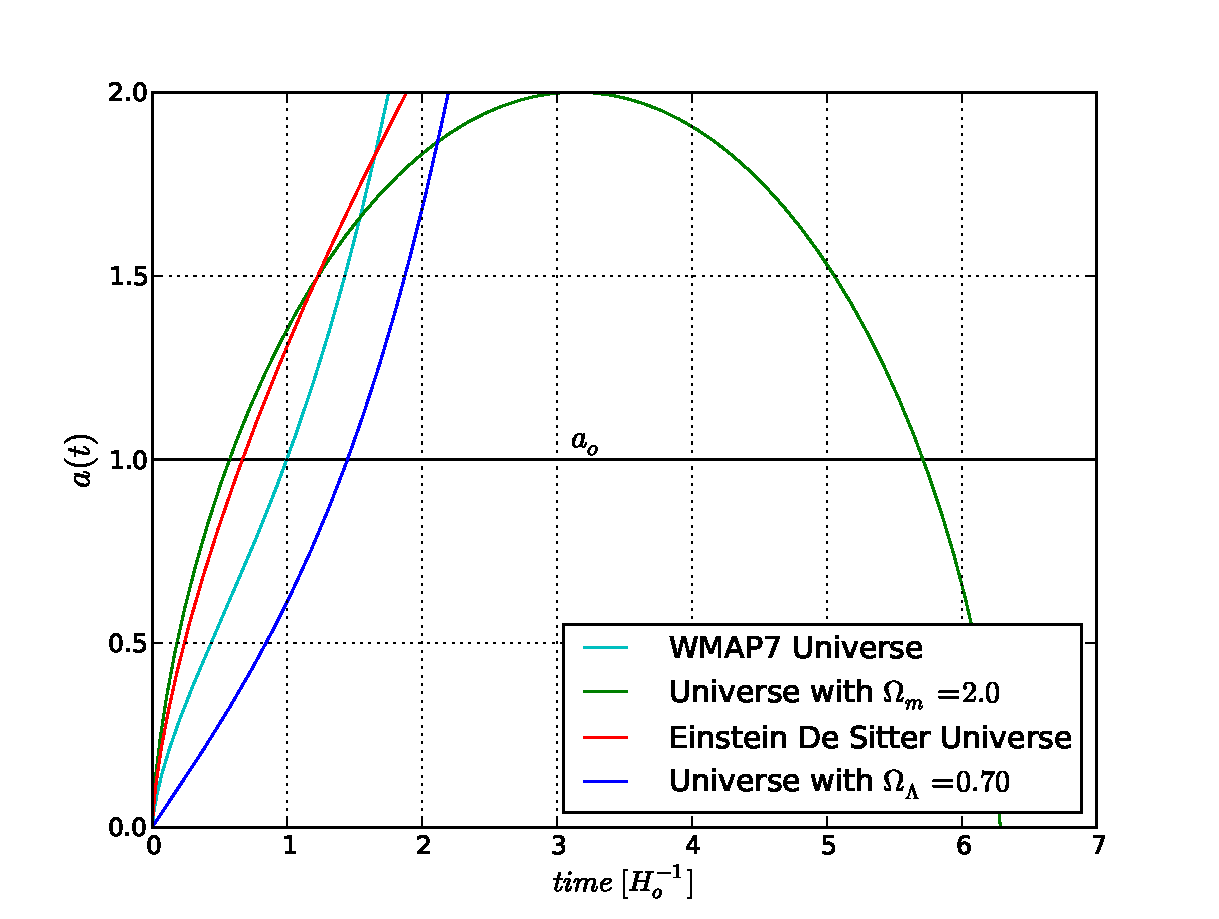
\includegraphics[width=0.8\textwidth]{Images/chapter2/factordeescala.pdf}
       \caption{ \small Scale factor as a time function. The Universe expansion for 
       different density contributions. A closed Universe is obtained when 
       $\Omega_m = \Omega_o>1$. Also, the WMAP7 parameters show an acelerated expansion. 
        }
       \label{factor}
 \end{figure}
%**********************************************************************************************************************

%&&&&&&&&&&&&&&&&&&&&&&&&&&&&&&&&&&&&&&&&&&&&&&&&&&&&&&&&&&&&&&&&&&&&&&&&&&&&&&&&&&&&&&&&&&&&&&&&&&&&&&&&&&&&&&&&&&&&&&
\section{Hilbert Einstein field equation}
%&&&&&&&&&&&&&&&&&&&&&&&&&&&&&&&&&&&&&&&&&&&&&&&&&&&&&&&&&&&&&&&&&&&&&&&&&&&&&&&&&&&&&&&&&&&&&&&&&&&&&&&&&&&&&&&&&&&&&&

At big scales, the most important fundamental interaction is the 
gravitational. Hence, the theory of general relativity (TGR) is 
an essential tool in the study of the cosmos. 

At smaller scales, the Newtonian gravitational theory is valid, where, 
the Poisson equation offers a relation between the second derivative
of the field and the source of the field 

\[ \nabla^2\Phi=4\pi G\rho\]

this equation is obtained from TGR for low velocities and 
a weak gravitational field ($\Phi/c^2<< 1$). A key equation of TGR is
the Hilbert-Einstein field equation


\eq{
R_{\mu\nu}-\f{1}{2}g_{\mu\nu}R-g_{\mu\nu}\Lambda = \f{8\pi G}{c^4}T_{\mu\nu}
}

a 6 independent component tensorial equation. The first term of the left
is Ricci tensor (second derivatives of the metric tensor). The second one 
is the scalar curvature that 

	

%&&&&&&&&&&&&&&&&&&&&&&&&&&&&&&&&&&&&&&&&&&&&&&&&&&&&&&&&&&&&&&&&&&&&&&&&&&&&&&&&&&&&&&&&&&&&&&&&&&&&&&&&&&&&&&&&&&&&&&
\section{ Friedmann equations }
%&&&&&&&&&&&&&&&&&&&&&&&&&&&&&&&&&&&&&&&&&&&&&&&&&&&&&&&&&&&&&&&&&&&&&&&&&&&&&&&&&&&&&&&&&&&&&&&&&&&&&&&&&&&&&&&&&&&&&&



%&&&&&&&&&&&&&&&&&&&&&&&&&&&&&&&&&&&&&&&&&&&&&&&&&&&&&&&&&&&&&&&&&&&&&&&&&&&&&&&&&&&&&&&&&&&&&&&&&&&&&&&&&&&&&&&&&&&&&&
\section{ State equation }
%&&&&&&&&&&&&&&&&&&&&&&&&&&&&&&&&&&&&&&&&&&&&&&&&&&&&&&&&&&&&&&&&&&&&&&&&&&&&&&&&&&&&&&&&&&&&&&&&&&&&&&&&&&&&&&&&&&&&&&




%&&&&&&&&&&&&&&&&&&&&&&&&&&&&&&&&&&&&&&&&&&&&&&&&&&&&&&&&&&&&&&&&&&&&&&&&&&&&&&&&&&&&&&&&&&&&&&&&&&&&&&&&&&&&&&&&&&&&&&
\section{ Perturbation evolution in the newtonian regimen }
%&&&&&&&&&&&&&&&&&&&&&&&&&&&&&&&&&&&&&&&&&&&&&&&&&&&&&&&&&&&&&&&&&&&&&&&&&&&&&&&&&&&&&&&&&&&&&&&&&&&&&&&&&&&&&&&&&&&&&&

%######################################################################################################################
\subsection{ Newtonian description  }
%######################################################################################################################
%######################################################################################################################
\subsection{ Jeans Inestability}
%######################################################################################################################



%&&&&&&&&&&&&&&&&&&&&&&&&&&&&&&&&&&&&&&&&&&&&&&&&&&&&&&&&&&&&&&&&&&&&&&&&&&&&&&&&&&&&&&&&&&&&&&&&&&&&&&&&&&&&&&&&&&&&&&
\section{ Statistical properties of cosmological perturbations }
%&&&&&&&&&&&&&&&&&&&&&&&&&&&&&&&&&&&&&&&&&&&&&&&&&&&&&&&&&&&&&&&&&&&&&&&&&&&&&&&&&&&&&&&&&&&&&&&&&&&&&&&&&&&&&&&&&&&&&&
%######################################################################################################################
\subsection{ Gaussian Random fields }
%######################################################################################################################
%######################################################################################################################
\subsection{ Linear perturbation spectrum }
%######################################################################################################################
%-----------------------------------------------------------------------------------------------------------
\subsubsection{ Initial power spectrum }
%-----------------------------------------------------------------------------------------------------------
%-----------------------------------------------------------------------------------------------------------
\subsubsection{ Amplitude of the linear power spectrum }
%-----------------------------------------------------------------------------------------------------------
%-----------------------------------------------------------------------------------------------------------
\subsubsection{ Standard deviation }
%-----------------------------------------------------------------------------------------------------------



%&&&&&&&&&&&&&&&&&&&&&&&&&&&&&&&&&&&&&&&&&&&&&&&&&&&&&&&&&&&&&&&&&&&&&&&&&&&&&&&&&&&&&&&&&&&&&&&&&&&&&&&&&&&&&&&&&&&&&&
\section{ Higher order perturbation theory }
%&&&&&&&&&&&&&&&&&&&&&&&&&&&&&&&&&&&&&&&&&&&&&&&&&&&&&&&&&&&&&&&&&&&&&&&&&&&&&&&&&&&&&&&&&&&&&&&&&&&&&&&&&&&&&&&&&&&&&&
%######################################################################################################################
\subsection{ Zeldovich approximation }
%######################################################################################################################


%&&&&&&&&&&&&&&&&&&&&&&&&&&&&&&&&&&&&&&&&&&&&&&&&&&&&&&&&&&&&&&&&&&&&&&&&&&&&&&&&&&&&&&&&&&&&&&&&&&&&&&&&&&&&&&&&&&&&&&
\section{ Cosmic density field }
%&&&&&&&&&&&&&&&&&&&&&&&&&&&&&&&&&&&&&&&&&&&&&&&&&&&&&&&&&&&&&&&&&&&&&&&&&&&&&&&&&&&&&&&&&&&&&&&&&&&&&&&&&&&&&&&&&&&&&&
%######################################################################################################################
\subsection{ Correlation functions }
%######################################################################################################################
%######################################################################################################################
\subsection{ Mass moments }
%######################################################################################################################
%######################################################################################################################
\subsection{ Clustering in the real and redshift space }
%######################################################################################################################
%-----------------------------------------------------------------------------------------------------------
\subsubsection{ Redshift distortions }
%-----------------------------------------------------------------------------------------------------------
%-----------------------------------------------------------------------------------------------------------
\subsubsection{ Real space correlation functions }
%-----------------------------------------------------------------------------------------------------------

%&&&&&&&&&&&&&&&&&&&&&&&&&&&&&&&&&&&&&&&&&&&&&&&&&&&&&&&&&&&&&&&&&&&&&&&&&&&&&&&&&&&&&&&&&&&&&&&&&&&&&&&&&&&&&&&&&&&&&&
\section{ Baryonic acoustic oscillations }
%&&&&&&&&&&&&&&&&&&&&&&&&&&&&&&&&&&&&&&&&&&&&&&&&&&&&&&&&&&&&&&&&&&&&&&&&&&&&&&&&&&&&&&&&&&&&&&&&&&&&&&&&&&&&&&&&&&&&&&
